%%%%%%%%%%%%%%%%%%%%%%%%%%%%%%%%%%%%%%%%%%%%%%%%%%%%%%%%%%%%%%%%%%%%%%%%%%%%%%%%
\documentclass[twocolumn]{revtex4}

%%%%%%%%%%%%%%%%%%%%%%%%%%%%%%%%%%%%%%%%%%%%%%%%%%%%%%%%%%%%%%%%%%%%%%%%%%%%%%%%
% Note that comments begin with a "%" and are not turned into text in the .pdf
% document.
%%%%%%%%%%%%%%%%%%%%%%%%%%%%%%%%%%%%%%%%%%%%%%%%%%%%%%%%%%%%%%%%%%%%%%%%%%%%%%%%

%%%%%%%%%%%%%%%%%%%%%%%%%%%%%%%%%%%%%%%%%%%%%%%%%%%%%%%%%%%%%%%%%%%%%%%%%%%%%%%%
% Include some extra packages.
%%%%%%%%%%%%%%%%%%%%%%%%%%%%%%%%%%%%%%%%%%%%%%%%%%%%%%%%%%%%%%%%%%%%%%%%%%%%%%%%
\usepackage{graphicx}
%%%%%%%%%%%%%%%%%%%%%%%%%%%%%%%%%%%%%%%%%%%%%%%%%%%%%%%%%%%%%%%%%%%%%%%%%%%%%%%%

%%%%%%%%%%%%%%%%%%%%%%%%%%%%%%%%%%%%%%%%%%%%%%%%%%%%%%%%%%%%%%%%%%%%%%%%%%%%%%%%
\begin{document}

%%%%%%%%%%%%%%%%%%%%%%%%%%%%%%%%%%%%%%%%%%%%%%%%%%%%%%%%%%%%%%%%%%%%%%%%%%%%%%%%
\title{Using Monty Carlo Methods to predict rain patterns}

\author{Matthew Johnson}
\affiliation{Siena College, Loudonville, NY}

\date{\today}

\begin{abstract}
   

In this project the analytical and numerical approach to finding the chance of rain in a month were compared. The first example was find the odd of only one day having rain in any given month when there is a twenty percent chance of rain on a given day. When using the analytical approach the chance or rain was calculated to be 0.9 percent and as expeceted the numerical approach gave around 0.9 percent. This was expected since both should give around the same result. The next part involved decreasing the chance of it raining to ten percent and finding what were the chances of it raining more than eight days in a month. The odds were that there is a 0.7 perecnt chance of it raining more than eight days.   Then using the numerical or Monty Carlo approach the chance for it rain more than 10 cm in a given month  was calculated which was around 65$\%$  .  Then using the rainfall values from the previius step a histogram was made which is shown in the section about question3 b. Then the average amount of rain fall in a given month was caluculated by taking adding all the values for rain in a set of months and diding by the amount of montths. This gave an answers of around 12 cm of rain every month.
\end{abstract}

\maketitle
%%%%%%%%%%%%%%%%%%%%%%%%%%%%%%%%%%%%%%%%%%%%%%%%%%%%%%%%%%%%%%%%%%%%%%%%%%%%%%%%

%%%%%%%%%%%%%%%%%%%%%%%%%%%%%%%%%%%%%%%%%%%%%%%%%%%%%%%%%%%%%%%%%%%%%%%%%%%%%%%%
\section{Introduction}
In this part of the document i will explain what the code is doing list and relevant funtions and show data from plots
\section{Question 1}
In this question I was tasked to calculate the odds of it raining one only one day a month when there is a 20$\%$ chanve it will rain any given day using two methods. The first method was to solve it analytically using formulas to give an exact value and second was to solve numericaly to find a value close to what the real value is. 
\subsection{Analyitical Method}
The anaytical method involes the use of this formula 
$$P(\textrm{total}) = P_{\textrm{1}} \times P_{\textrm{2}} $$
Which is the formula used when something and somelese happens. 
So to solve this  a function was made that calculated the odd of it rain on only one day. This was done by putting 0.2 to the power of the days in which it ains which is one. The chance of it not raining is $1-0.2=0.8$ and that put to the power of the days it did not rain 29. Then the result was multipled by 100 to convert into percent. However that only gave the reult of the first day rain what happens if the second day rains. The function is the same and you would have to add a value for every day of the month however since the values are the same you can multiply by the amount of days to get the answer 0.93$\%$. 

\subsection{Numerical}
In this section a Monty Carlo method was used solve the question. This is done by generating a bunch of random numbers and using them to solve the question. The first step was making a function called rain day() that said whether it rained or not. This was done by generating a random number between 0 and 1 using the$ random.random() $function from numpy. If the number was under 0.2 it rained and the function gave a output of 1. If the value was bigger than 0.2 the function returned a zero.

Then the result of that function was passed into the function called $ daysitrain()$ whichdefualted to run $  rainday() $ 30 times representing a month. All the outputs were added which gave the number of days it rained in that month. 

Then to get the percentage of months were it rained once the function $month1rain()$ was made. This function was defauled to run 10,000 times to simuluate 10,000 months. A for statement was used the  the function$ daysitrain()$ and whenever that function returned a value of one it added 1 to $ one_rain$  a number that starts at zero. Then that value was divided by the amount of months and multiplied by 100 to give a percentage. That gave a number ranging around 0.9$\%$.
%%%%%%%%%%%%%%%%%%%%%%%%%%%%%%%%%%%%%%%%%%%%%%%%%%%%%%%%%%%%%%%%%%%%%%%%
\section{Question 2}
In question two the question was to solve for  the odds that it would rain more than 8 days when the chance for rain is 10$\%$. 
The Monty Carlo method was used again witht eh same method as before. There were only two values changed rain day was changed so when the random.random function gives a value less than 0.1 does 1 get added to rain and in month one rain the values was chaged to greater then eight to add one to one rain. The rest was the same as before. This gave a value of around 0.7$\%$

\section{Question 3}
\subsection{3a}
In this question the odd that it would gain more than 10 cm in any given month was calulated. This was done by using a series of equations that reprented differnt variables. The rain day functions used the modifed rain rates to calculate if it will rain or not. Rain day is used when there was no rain the previous day and the chance of rain  is 10 $\%$. Rain day 2 is used  when 1 day before but not two so it is a 20$\%$ chance of rain. Rain day 3 is when it rained the last two days but not three and that has a 25$\%$ chance of rain. Lastly rain day 4 is when it rained three or more days in a row and that has a 5$\%$ chance of rain.  The last function that was made was amt rain this function would determine the amout of rain when it rains. This works from that all possibilites will add up to one. The range of each term represents the percent odds of each rain fall.  The upper bound is a whole number since the values are given in whole numbers. Anything greater will be the next perecnt bracket. 

Then a function was made called will it rain that loops through 30 different days. To do this two list are made days keeps track of it it rained and rainamt keeps track of the amount of rain.  In the third for loop days it rained was deermined. To start of the for loop some terms had to calulated seperately. For the first second and third  day due to the constrains of the quetion the function would have went out of range if it tried to look back three days. The forth day was calculated seperately just in case i counted wrong  so it would not be potentially out of bounds. After each time i was increased by one to continue the loop. Then at i  greater than or equal to 5 the function operateed normally. When all day equal 1 that represents it raining for the last three days. In this case rain day 4 is used. When days  i =3 is zero but the other days terms are 1 the represents it raining the last two days.In this case rain day 3 is used. When days i-3 and days i-2 =0 and days i-1 is one that represents it raining the last day only. In this case rain day 2 is used.When all days equal 0 that represents haing no days of rain and rain day is used.
Any time all the values in the if statement are true the day value at that i term is set to 1 and rainamt is used which replaces the value of rain amount with the generated rain value at that i term. Then the function returns the sum of rainamt which is the amount it rained that month.
Then to find the odds that it rains more than 10 cm of rain the will it rain is ran 10000 times to test for a large amount of months. It is rain in a if staement which says that anythie it rains more than 10 cm add 1 to a term called one rain which was preset at zero. The function returns a number which is then divide by the amount of months times 100 to give the percentage of months where it rains more than 10 cm which is around 65$\%$
\subsection{3b}
In this question a histogram is made from the rainfall values from the function will it rain after it is ran 10000 times in a for loop. On the histogram the x value is the amount of rain and the y is how many times those values occured.  The polt size is from fig size and the range is set to 39 since values ranged from 0 to 39.  The amount of bins is the amount of columns.  Which is shown in the figure below
\begin{figure}[h] 
\centering
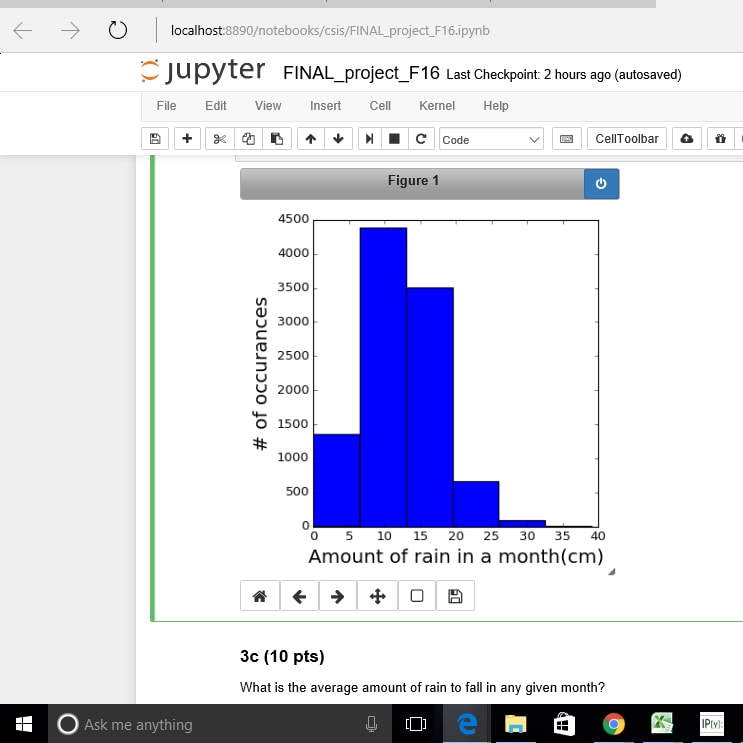
\includegraphics [width=0.5\textwidth]{pic.jpg}{\hspace{0.5 in}}
\caption{ This is the histogram of rain values\label{Histogram}}
\end{figure}


\subsection {3c}
In this question the average rainfall value was found. This was found by adding all the rain values from each month and diving by the amount of months in a for loop. 

The function for average is  
$$\frac{n1+n2+nn}{n}=average$$
%%%%%%%%%%%%%%%%%%%%%%%%%%%%%%%%%%%%%%%%%%%%%%%%%%%%%%%%%%%%%%%%%%%%%%%%%%%%%%%%

%%%%%%%%%%%%%%%%%%%%%%%%%%%%%%%%%%%%%%%%%%%%%%%%%%%%%%%%%%%%%%%%%%%%%%%%%%%%%%%%

%%%%%%%%%%%%%%%%%%%%%%%%%%%%%%%%%%%%%%%%%%%%%%%%%%%%%%%%%%%%%%%%%%%%%%%%%%%%%%%%
\end{document}
%%%%%%%%%%%%%%%%%%%%%%%%%%%%%%%%%%%%%%%%%%%%%%%%%%%%%%%%%%%%%%%%%%%%%%%%%%%%%%%%
